% !TEX root = ../VPJ.tex

\chapter{Einleitung}
\label{sec:Einleitung}

Um an einem realen System Abläufe und Prozesse zu simulieren, wird den Studierenden eine Anlage zur Verfügung gestellt, welche hauptsächlich aus Teilen der Firma „Festo“ besteht (folgend: Festo-Transfersystem). An diesem Festo-Transfersystem können die Studierende Laufbänder, Ampelanlage, Lichtschranken, Weichen etc. mithilfe selbst geschriebener Programme ansteuern und auslesen. 

Das Laufband kann aufgelegte Objekte transportieren. Dabei kann die aktuelle Position des Objekts durch diverse Lichtschranken erfasst werden. Am Anfang des Laufbands kann mithilfe eines Entfernungssensors die Höhe des Objekts erfasst werden. Mit den vorhandenen Komponenten kann das Festo-Transfersystem allerdings ausschließlich die Position und die Höhe der Objekte bestimmen und nicht deren Farbe, Form, Ausrichtung oder sonstige optische Merkmale. 

\begin{figure}[htb]
    \centering
    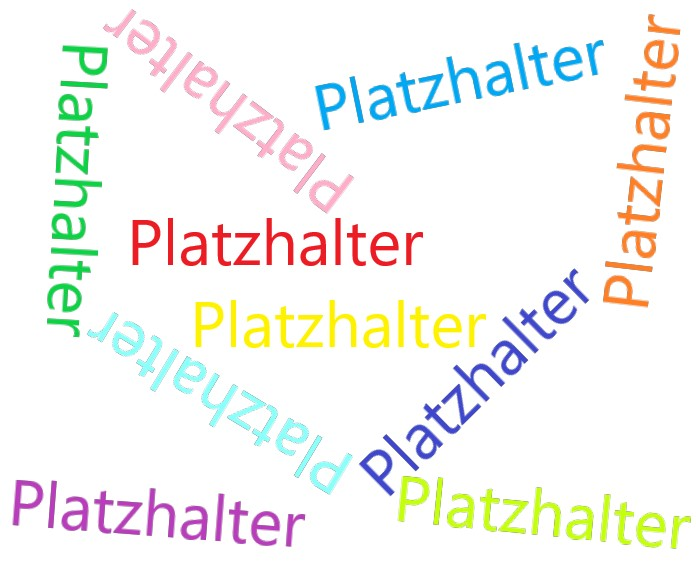
\includegraphics[width=0.6\textwidth]{Abbildungen/Platzhalter.jpg}
    \caption[CMUcam5 Pixy \newline Quelle: \textit{http://charmedlabs.com/default/products/}]{CMUcam5 Pixy}		
    \label{fig:PixyCam}
\end{figure}

Eine Erweiterung um ein Kamerasystem kann diese Mängel beheben und sogar noch weitere Funktionen und Features hinzufügen. 

\section{Vorhaben}
\inlinetodo {blabla}
Ähnlich einer Smart Kamera \cite{festo_dok}, bei der nicht nur das Kamerabild, sondern auch weitere schon verarbeitete Informationen ausgegeben werden sollen, wird ein Prozessor benötigt, welcher in der Lage ist Bildverarbeitung durchzuführen. Es wurde als Möglichkeit für ein Prozessorsystem empfohlen, sich mit dem BeagleBone Black und Raspberry PI auseinanderzusetzen. Mithilfe einer Marktrecherche werden zunächst weitere geeignete Kamerasysteme gesucht und anschließend anhand der Eignung sortiert. Dabei wird auch eine geeignete Schnittstelle zu dem Kamerasystem ausgewählt, mit dem die Bilder und Informationen an den PC gesendet werden. Nachdem die beiden geeignetsten Kamerasysteme gewählt und bestellt sind, werden zugehörige Gehäuse und Befestigungen konstruiert und gefertigt. Nebenbei werden erste einfache Testprogramme geschrieben, um die Funktion von den gewählten Kamerasystemen zu gewährleisten. Der erste Prototyp wird dabei voraussichtlich mit Hilfe rapid-prototyping ein Erzeugnis aus dem 3D-Druck sein, um Kamera an der richtigen Position zu halten. Nachdem das Endprodukt montiert ist, folgt eine Auswertung der Kamerabilder. Folgend folgen optional das Erstellen einer Bibliotheksdatei und eine Automation der Kalibrierung und des Weißabgleichs. Der Zugriff auf die Kamera soll gewährleistet sein. 

\begin{figure}[htb]
    \centering
    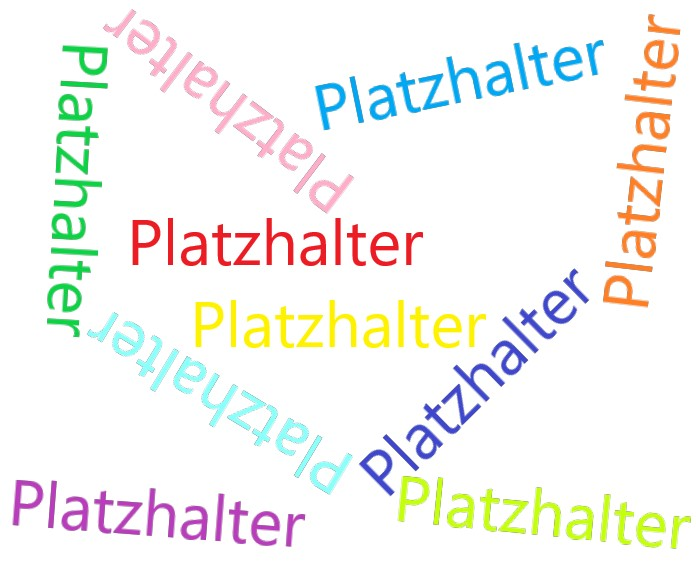
\includegraphics[width=0.4\textwidth]{Abbildungen/Platzhalter.jpg}
    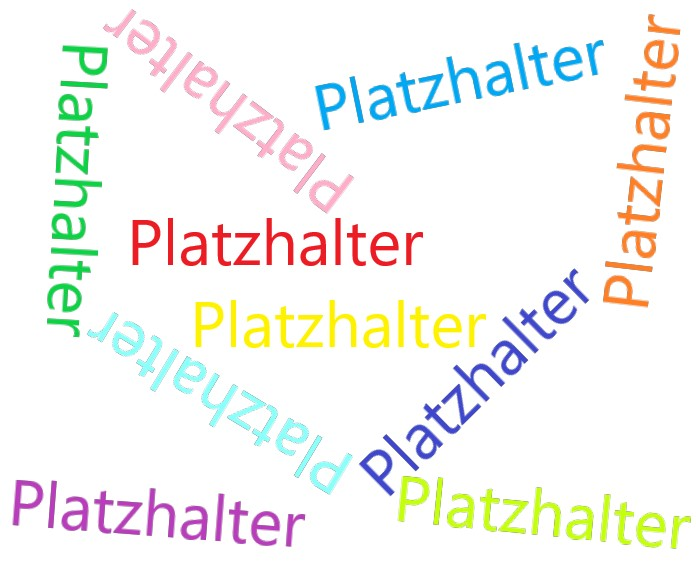
\includegraphics[width=0.4\textwidth]{Abbildungen/Platzhalter.jpg}
    \caption{PixyCam Gehäusefehler}		
    \label{fig:Pixy_Fehler}
\end{figure}

